\documentclass{beamer}
\usepackage{tikz}
\usetikzlibrary{positioning, shapes.geometric, arrows.meta, fit, calc}

\usetheme{Madrid} % Choose a theme (e.g., Madrid, AnnArbor, Berkeley, etc.)
\usecolortheme{dolphin} % Choose a color theme (optional)

\title{Fake News Classification}
\author{
  \begin{tabular}{l l}
    Shasank Reddy Pinnu & 23b1015 \\
    Sree Vamshi Madhav Nenavath & 23b1039 \\
  \end{tabular}
}
\date{\today}

\setbeamertemplate{footline}{}


\begin{document}

\frame{\titlepage} % Title slide

\begin{frame}
    \frametitle{Introduction \& Problem Statement}
    This Project of Fake news detection involves classifying articles as \textbf{Real} or \textbf{Fake} based on their content. 
    
    \vspace{0.3cm}
    \textbf{Input Format:} Textual content including the \textbf{Title} and \textbf{Body} of the article. 
    
    \vspace{0.3cm}
    \textbf{Output:} 
    \begin{itemize}
        \item \textbf{Real:} Verified true news.
        \item \textbf{Fake:} False or misleading news.
        \item \textbf{Fake News Subclassification:} Further classification of fake news into categories.
    \end{itemize}
\end{frame}

\begin{frame}
\frametitle{Example}
\textbf{Input:} 
    \begin{description}
        \item[Title:] {\scriptsize\texttt{The 9/11 Commission Didn't Believe the Government… So Why Should We?}}
        \item[Body:] {\scriptsize\texttt{
            9/11 Commissioners Admit They Never Got the Full Story The 9/11
            Commissioners publicly expressed anger at cover ups and obstructions
            of justice by the government into a real 9/11 investigation: ...
        }}
    \end{description}

\textbf{Output:}
    \begin{itemize}
        \item \textbf{Classification:} \texttt{Fake}
        \item \textbf{Fake News Subclassification:} \texttt{Conspiracy Theory}
    \end{itemize}
\end{frame}

\begin{frame}
    \frametitle{Motivation}
    
    \vspace{0.5em}
    \textbf{Relevance:}
    \begin{itemize}
        \item The widespread growth of online misinformation and fake news undermines public trust and informed decision-making.
    \end{itemize}
    
    \vspace{1em}
    \textbf{Why This Problem is Interesting:}
    \begin{itemize}
        \item Involves real-world impact combined with natural language processing.
        \item Addresses societal challenges using machine learning techniques.
    \end{itemize}
    
    \vspace{0.5em}
    \textbf{Applications:}
    \begin{itemize}
        \item Fake news detection tools to assist media platforms and users.
        \item Automated fact-checking systems.
        \item Educational platforms for promoting media literacy.
    \end{itemize}
    
\end{frame}
    
    
\begin{frame}
    \frametitle{Prior Work and Inspiration}
    
    \textbf{Paper:} \textit{A Fake News Detection System based on Combination of Word Embedded Techniques and Hybrid Deep Learning Model} \\
    \textbf{Authors:} M. A. Ouassil et al. (IJACSA, 2022)
    
    \vspace{0.2cm}
    \textbf{Summary:}
    \begin{itemize}
        \item Used a CNN-BiLSTM hybrid model for fake news detection.
        \item Combined CBOW and Skip-Gram Word2Vec embeddings.
        \item Evaluated on WELFake dataset with 97.74\% accuracy.
    \end{itemize}
    
    \vspace{0.2cm}
    \textbf{Inspiration for Our Approach:}
    \begin{itemize}
        \item Hybrid CNN-BiLSTM for learning local + sequential features.
        \item Framework adaptable for subclassifying fake news (e.g., conspiracy, satire).
    \end{itemize}
    
\end{frame}
    

\begin{frame}{Dataset Overview}
    \begin{itemize}
        \item \textbf{Data Format:}
        \begin{itemize}
            \item Each instance includes: \texttt{type}, \texttt{title}, \texttt{content}, and \texttt{label}
            \tiny
            \begin{tabular}{|c|p{2cm}|p{3.2cm}|c|}
                \hline
                \textbf{Type} & \textbf{Title (truncated)} & \textbf{Content (truncated)} & \textbf{Label} \\
                \hline
                conspiracy & The 9/11 Commission Didn’t Believe... & 9/11 Commissioners Admit They Never... & 1 \\
                clickbait & Former Watergate Prosecutors:... & 5545 SHARES Facebook Twitter... & 1 \\
                hate & Hindu Group Criticizes Toronto... & A Hindu group that regularly... & 1 \\
                \hline
            \end{tabular}
            \normalsize
    
        \end{itemize}
        
        

        
        \vspace{0.4cm}
        
        \item \textbf{Dataset Statistics:}
        Due to the large size of the dataset, we used a subset of the data for our experiments.
        \begin{itemize}
            \item Total Samples: \textbf{110,000}
            \item Total classes: \textbf{11} (10 types of \textit{fake}, 1 \textit{real}) 10,000 samples per class.
            \item Training samples: \textbf{99,000}
            \item Test samples: \textbf{11,000}
        \end{itemize}

        \item \textbf{Source:} \url{https://github.com/several27/FakeNewsCorpus/}
    \end{itemize}
\end{frame}

\begin{frame}{Model Architecture}
    \begin{itemize}
        % \item for Text Embeddings, Pre-trained \texttt{GloVe (Global Vectors for Word Representation)} embeddings used.
        % \begin{itemize}
        %     \item 100-dimensional vectors.
        %     \item Captures semantic similarity based on co-occurrence statistics from a large corpus (Wikipedia + Gigaword).
        % \end{itemize}
        
        \item For the two tasks, we trained two separate models.
        \begin{itemize}
            \item \textbf{\textcolor{structure}{Primary Classifier}:} Classifies articles as \textbf{Real} or \textbf{Fake}.
            \item \textbf{\textcolor{structure}{Secondary Classifier}:} Classifies \textbf{Fake} articles into 10 categories.
        \end{itemize}

        \item Both models share the same architecture with the following components:
        \begin{itemize}
            \item \textcolor{structure}{GloVe Encoder:} Converts text into 100-dimensional GloVe embeddings.
            \item \textcolor{structure}{CNN Layers:} Extract local n-gram features from input embeddings.
            \item \textcolor{structure}{BiLSTM:} Captures sequential dependencies in both directions (forward and backward).
        \end{itemize}
        
        \item They only differ at the final Fully Connected (FC) layers, where the number of output classes varies.
        
        \item The overview of the architecture is:
        \vspace{0.5cm}

        \begin{center}
        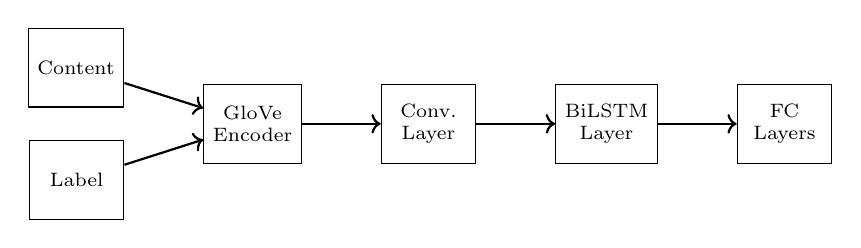
\begin{tikzpicture}[
            box/.style={
                rectangle,
                draw=black,
                minimum height=1cm,
                minimum width=1.2cm,
                align=center,
                font=\scriptsize
            },
            arrow/.style={->, thick}
        ]

        % Nodes
        \node[box] (Encoder) {GloVe\\Encoder};
        \node[box, above left=-0.3cm and 1cm of Encoder] (Input) {Content};
        \node[box, below left=-0.3cm and 1cm of Encoder] (Label) {Label};
        \node[box, right=1cm of Encoder] (CNN) {Conv.\\Layer};
        \node[box, right=1cm of CNN] (LSTM) {BiLSTM\\Layer};
        \node[box, right=1cm of LSTM] (FC) {FC\\Layers};

        % Arrows
        \draw[arrow] (Input) -- (Encoder);
        \draw[arrow] (Label) -- (Encoder);
        \draw[arrow] (Encoder) -- (CNN);
        \draw[arrow] (CNN) -- (LSTM);
        \draw[arrow] (LSTM) -- (FC);

        \end{tikzpicture}
        \end{center}
        
    \end{itemize}
\end{frame}


\begin{frame}
\frametitle{Model Architecture}
    \begin{figure}[h!]
        \centering
        \scalebox{0.5}{ % Adjust this value to fit the diagram within the frame
        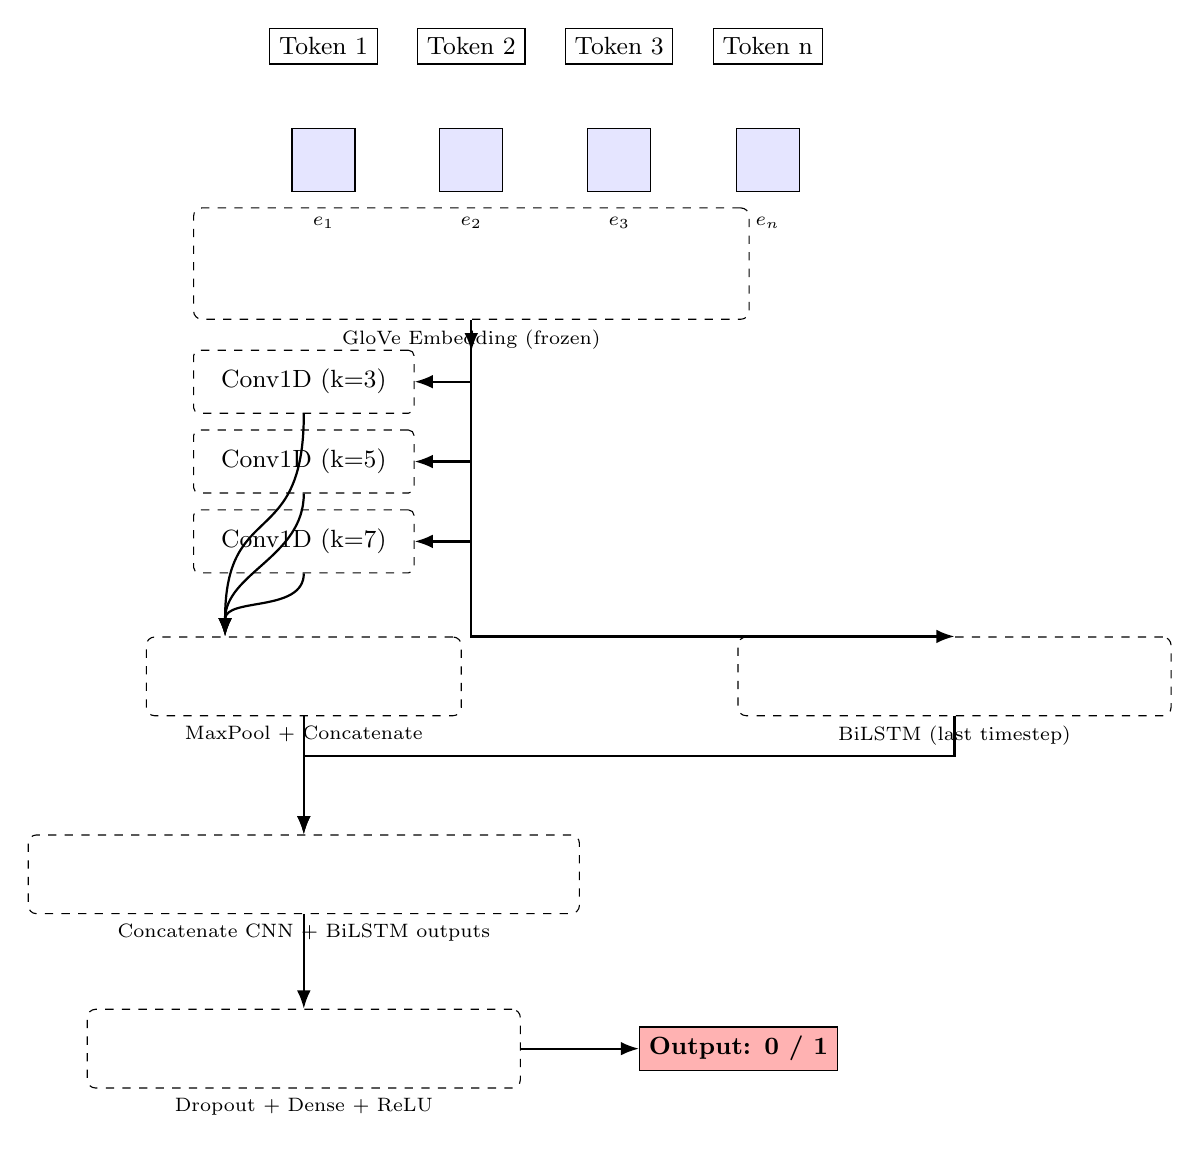
\begin{tikzpicture}[
            node distance=0.5cm and 0.5cm,
            token/.style={draw, minimum width=1cm, minimum height=0.4cm, align=center},
            vec/.style={draw, fill=blue!10, minimum height=0.8cm, minimum width=0.8cm},
            layer/.style={draw, dashed, inner sep=0.3cm, rounded corners=3pt, minimum height=1cm, minimum width=5.5cm},
            smalllayer/.style={draw, dashed, inner sep=0.2cm, rounded corners=2pt, minimum height=0.8cm, minimum width=2.8cm},
            arrow/.style={-Latex, thick},
            font=\small
        ]
        
        % Input Tokens
        \node[token] (tok1) {Token 1};
        \node[token, right=of tok1] (tok2) {Token 2};
        \node[token, right=of tok2] (tok3) {Token 3};
        \node[token, right=of tok3] (tok4) {Token n};
        
        % Embeddings
        \node[vec, below=0.8cm of tok1] (e1) {};
        \node[vec, below=0.8cm of tok2] (e2) {};
        \node[vec, below=0.8cm of tok3] (e3) {};
        \node[vec, below=0.8cm of tok4] (e4) {};
        
        \node at (e1.south) [yshift=-0.4cm] {\scriptsize $e_1$};
        \node at (e2.south) [yshift=-0.4cm] {\scriptsize $e_2$};
        \node at (e3.south) [yshift=-0.4cm] {\scriptsize $e_3$};
        \node at (e4.south) [yshift=-0.4cm] {\scriptsize $e_n$};
        
        % Embedding Label
        \node[layer, fit=(e1)(e4), below=0.2cm of e2, label=below:{\scriptsize GloVe Embedding (frozen)}] (embed) {};
        
        % CNN Branches
        \node[smalllayer, below=1.5cm of embed.west, anchor=west] (cnn3) {Conv1D (k=3)};
        \node[smalllayer, below=0.2cm of cnn3] (cnn5) {Conv1D (k=5)};
        \node[smalllayer, below=0.2cm of cnn5] (cnn7) {Conv1D (k=7)};
        
        % Arrows from Embedding to CNN
        % Midpoint anchor
        \coordinate (embedMid) at ($(embed.south) + (0,-0.4)$);
        
        \draw[arrow] (embed.south) -- (embedMid);
        \draw[arrow] (embedMid) |- (cnn3.east);
        \draw[arrow] (embedMid) |- (cnn5.east);
        \draw[arrow] (embedMid) |- (cnn7.east);
        
        
        % CNN Output join
        \node[layer, below=0.8cm of cnn7, minimum width=4cm, label=below:{\scriptsize MaxPool + Concatenate}] (cnnmerge) {};
        
        \draw[arrow] (cnn3.south) to[out=-90, in=90, looseness=1.5] ([xshift=-1cm]cnnmerge.north);
        \draw[arrow] (cnn5.south) to[out=-90, in=90, looseness=1] ([xshift=-1cm]cnnmerge.north);
        \draw[arrow] (cnn7.south) to[out=-90, in=90, looseness=1] ([xshift=-1cm]cnnmerge.north);
        % BiLSTM
        \node[layer, right=3.5cm of cnnmerge, label=below:{\scriptsize BiLSTM (last timestep)}] (bilstm) {};
        \draw[arrow] (embed.south) |- (bilstm.north);
        
        % Combine CNN + LSTM
        \node[layer, below=1.5cm of cnnmerge, minimum width=7cm, label=below:{\scriptsize Concatenate CNN + BiLSTM outputs}] (concat) {};
        \draw[arrow] (cnnmerge.south) -- (concat.north -| cnnmerge.south);
        \draw[arrow] (bilstm.south) -- ++(0,-0.5) -| (concat.north);
        
        % Dense + Dropout
        \node[layer, below=1.2cm of concat, label=below:{\scriptsize Dropout + Dense + ReLU}] (dense) {};
        \draw[arrow] (concat.south) -- (dense.north);
        
        % Output
        \node[draw, fill=red!30, right=1.5cm of dense] (pred) {\textbf{Output: 0 / 1}};
        \draw[arrow] (dense.east) -- (pred.west);
        
        % Caption for tokens
        \node[align=center, font=\footnotesize, below=4.7cm of tok2] at ($(tok2)!0.5!(tok3)$) {};
        
        \end{tikzpicture}
        }
        \caption{Architecture of CNN + BiLSTM model for Primary classification}
    \end{figure}
\end{frame}

\begin{frame}{Model Architecture Intuition}
    \begin{itemize}
        \item Two separate models are used to allow the LSTM layers to specialize in learning different feature patterns.
        \item The primary model focuses on separating real and fake samples, capturing generic semantic cues.
        \item The secondary model is trained only on fake samples, allowing it to specialize in distinguishing fine-grained patterns among fake types.
        \item Training models separately ensures that each LSTM captures task-specific temporal dependencies without interference.
        \item This setup improves feature disentanglement, reduces overfitting, and yields better generalization on both classification stages.
    \end{itemize}
\end{frame}

\begin{frame}{Implementation Details and Libraries}
    \textbf{\textcolor{structure}{Libraries:}}
    \begin{itemize}
        \item \texttt{torch}, \texttt{torch.nn}, \texttt{torchtext} – model and vocab handling
        \item \texttt{GloVe (6B, 100d)} – static embeddings via \texttt{torchtext.vocab}
        \item \texttt{scikit-learn, seaborn} – evaluation metrics (accuracy, F1, confusion matrix)
    \end{itemize}

    \textbf{\textcolor{structure}{Model Design (Shared):}}
    \begin{itemize}
        \item \texttt{Embedding:} GloVe-initialized, frozen
        \item \texttt{CNN:} Three 1D conv layers (kernel sizes 3, 5, 7), 100 filters each
        \item \texttt{BiLSTM:} Hidden size = \texttt{hidden\_dim}, bidirectional
        \item \texttt{Feature Vector:} Concatenated CNN + LSTM outputs $\rightarrow$ 400-D
    \end{itemize}

\end{frame}




\begin{frame}
    \frametitle{Results}
    
    \begin{itemize}
        \item \textbf{\textcolor{structure}{Primary Classifier:}} Achieved a high accuracy of \textbf{98\%}.
        
        \item \textbf{\textcolor{structure}{Secondary Classifier:}} Achieved \textbf{86\%} accuracy in identifying one of the 10 fake news types.
        
        \item \textbf{\textcolor{structure}{Single Unified Model Attempt:}} We also experimented with a single model trained jointly to perform both tasks.
        \begin{itemize}
            \item However, it could only reach around \textbf{80\%} accuracy.
            \item This underperformance highlights the difficulty in jointly optimizing for both coarse (real/fake) and fine-grained (type) classification.
        \end{itemize}
    \end{itemize}
    
\end{frame}
    

\begin{frame}
    \frametitle{Confusion Matrices}
    
    \begin{columns}
        \column{0.5\textwidth}
        Primary Classifier
        \vspace{1cm}
        \includegraphics[width=\linewidth]{images/primary_confusion_matrix.jpeg}

        \column{0.5\textwidth}
        Secondary Classifier
        \vspace{1cm}
        \includegraphics[width=\linewidth]{images/secondary_confusion_matrix.jpeg}
    \end{columns}
    
    \vspace{0.3cm}
    
\end{frame}

\begin{frame}{Model Analysis}

    \begin{itemize}
        \item \textbf{Justification for Two Separate Models:}
        \begin{itemize}
            \item Primary Model: 97\% accuracy
            \item Secondary Model (Subclass Classification): 86\% accuracy
            \item Combined accuracy of the two models:
            \[
            100 - 12 \times \left(\frac{1}{11}\right) - 14 \times \left(\frac{10}{11}\right) = 86.7\%
            \]
            which is higher than 80\%. This justifies the need for separate models as the features required for the primary classifier (real vs fake) and the secondary classifier (subcategories) may differ in the LSTM part.
        \end{itemize}
    \end{itemize}

    \vspace{0.5cm} % Adds space for the footer text

    \footnotesize
    \textit{Note:} $1/11$ and $10/11$ represent the fraction of real and fake data respectively.
    $12\%$ is the false negative accuracy of primary classsifer and
    $14\%$ is the inaccuracy of secondary model
    
\end{frame}


\begin{frame}{Model Analysis}
    \begin{itemize}
        \item \textbf{Primary Classifier Confusion Matrix Analysis:}
        \begin{itemize}
            \item Some true news articles are misclassified as fake ($12\%$) (False Negative).
            \item This could be due to the skewed ratio of the training data.
            \item No false articles are classified as true (True Negatives).
            \item This behavior is intentional, as the model is designed to be \textit{cynical} and err on the side of tagging content as fake.
        \end{itemize}

        \item \textbf{Secondary Classifier Confusion Matrix Analysis:}
        \begin{itemize}
            \item The main source of inaccuracy in the secondary classifier is in classifying articles into political, bias, and satire categories.
            \item These categories are more challenging for the model, as they share overlapping features and often involve subjective interpretation.
        \end{itemize}
        
    \end{itemize}

\end{frame}

\begin{frame}{Model Analysis}
    \begin{itemize}
        \item The Primary classifier achieves an accuracy of $\sim$97\%.
        \item This roughly matches the performance reported in the original paper (on the \texttt{WeLFake} dataset).
        \item Despite using a different dataset, similar results indicate strong generalization ability of the model.
    \end{itemize}
\end{frame}


\begin{frame}{Improvements Over Original Model}
    \begin{itemize}
        \item \textbf{Baseline (Paper's Model):}
        \begin{itemize}
            \item Performs only binary classification – detecting real vs fake.
            \item No capability to classify different types of fake samples.
        \end{itemize}

        \vspace{0.5em}
        \item \textbf{Our Two-Stage Architecture:}
        \begin{itemize}
            \item \textbf{Stage 1:} Binary classifier (Primary) detects fake vs real.
            \item \textbf{Stage 2:} Multi-class classifier (Secondary) classifies fake samples into subcategories.
        \end{itemize}

        \vspace{0.5em}
        \item \textbf{Advantages:}
        \begin{itemize}
            \item Specialized models improve precision and generalization.
            \item Better handling of fake subcategories due to focused training.
            \item Achieved $\sim$97\% accuracy in Stage 1 and $\sim$86\% in Stage 2.
        \end{itemize}
    \end{itemize}
\end{frame}

\begin{frame}{What We Learned}
    \begin{itemize}
        \item Understood the theory behind LSTMs and CNNs.
        \item Gained experience on how to improve model performance through trial
        and error and analysis, like
        \begin{itemize}
            \item testing SVM on the features from LSTM outputs,
            \item trying a single model for all 11 classes (fake + real), which led to inferior
            accuracy compared to the two-stage approach
        \end{itemize}
        \item Got comfortable with PyTorch and torchtext for building NLP models.
        \item Used scikit-learn for evaluation; accuracy, F1, confusion matrix.
        \item Built a simple UI with Streamlit to test the model live.
        
    \end{itemize}
\end{frame}

\end{document}
